%*****************************************
\chapter{Background}
\label{ch:background}
%*****************************************
%\hint{This chapter should give a comprehensive overview on the background necessary to understand the thesis.
%The chapter should have a length of about five pages!}

A joint base of concepts is necessary for the development of this thesis. This chapter aims to establish the fundamental ideas necessary to comprehend this thesis.
%As such a recap can never be totally comprehensive prerequisites are %unavoidable. 
%The most notable are:
%\begin{itemize}
	%\item Understanding the concept of over-fitting
	%\item ...
%\end{itemize}

\section{Neural Networks}

Neural networks are a part of most breakthroughs in artificial intelligence over the last decade enabling computers to
compete in fields formerly championed by humans.\footnote{\begin{itemize}[topsep=0pt]
		\item 
		2011: "Watson" of IBM defeats two former grand champions in "Jeopardy!" \cite{lally2011natural}
		\item 
		2011: "Siri" enables users to use natural language to interact with their phones 
		\cite{ARON201124}
		\item 
		2015: A convolutional neural network classifies images from the ImageNet dataset more accurately than humans 
		\cite{Russakovsky2015} \cite{He_2015_ICCV}
		\item 
		2016: "AlphaGo" beats Lee Sedol, one of the world's strongest Go players
		\cite{gibney2016google} \cite{silver2017mastering}
	\end{itemize}
} They implement a statistical approach to \textbf{supervised learning},
which is to say that they try to find a specific model optimizing the likelihood of reproducing input-output pairs similar to some training data. In contrast to other approaches, which directly divine behavior rules from expert knowledge, they are far more dependant on any training data.\cite{Statistical-ML-Basics}\\
Apart from the provided data, the essential point of the design is the class of all possible models the approach could represent after training. A multitude of properties are usually sought in a model class of which a few important ones are:
\begin{itemize}
	\item \textbf{Richness:}\\
	The diversity of single models in the class and thus the ability to fit a wide field of different input-output landscapes.\footnote{More formally the richness of a model class can be described as the amount of different functions from the input-space to the output-space which can be expressed through any model of said class.}\\
	A model class lacking richness is inherently restricted, and thus the underlying mapping between inputs and outputs might be beyond the expressive capabilities of all its models.\\
	In other words: If a model class is not rich enough, all of its models will fail to represent the given training data appropriately. This phenomenon is called \textbf{underfitting}.
	\item \textbf{Stability:}\\ 
	The tendency of similar models in the class to handle inputs similarly.
	If a model class shows unstable behavior, defining a sensible way to search it for good models becomes difficult.
	\item \textbf{Interpretability of Models:}\\
	Interpretability expresses the ease of formulating knowledge about a task given a well-performing model of the class.
	As fields exist in which statistical approaches outperform experts, the extraction of knowledge understandable and applicable by humans is of particular interest.
\end{itemize}
If one knows an entity that already performs well on a given task, it is a sensible approach to design one's model class to reproduce its decision process. Humans usually embody such entities for many tasks of interest in real-world applications, so they are a natural source of inspiration. In a nutshell, neural networks are simplified models of a human central nervous system.\\

\subsection{Basics}
The most fundamental building block of the human central nervous system is a \textbf{neuron} that can receive multiple stimuli and can produce an output if the combined stimulation exceeds a threshold. Figure \ref{fig:neuron1} depicts one such neuron and its stimulus measure. Another functionality observed in nature is the ability of a neuron to strengthen the connection to any source of stimulus, thus giving said source more influence on whether the neuron produces an output.\cite{Biology_Background}\\
\\
The canonical mathematical model of a neuron, as seen in \ref{fig:neuron2}, is defined as:
\begin{itemize}
	\item \textbf{Inputs} $x_i$\\
	All stimuli of a neuron are either referred to as its inputs or as the \textbf{features} of the data.\\
	\item \textbf{Weights} $w_i$\\
	The ability to assign importance to specific stimuli is modeled as weights.\\
	\item \textbf{Combined Weighted Inputs} $\sum_{i=1}^{n}w_i x_i$\\
	A summation superposes the inputs, scaled according to their respective weight, to form the total excitation of the neuron.\\
	\item \textbf{Activation Function} $\Phi(\sum_{i=1}^{n}w_i x_i)$\\
	The monotonously ascending activation function defines the Correlation between excitation of the neuron and its output signal.\\
	\item \textbf{Bias} $b$\\  
	As different neurons display varying thresholds of activation, the previously mentioned summation includes an input independent base term. This term effectively shifts the activation of the modeled neuron.\\
\end{itemize}

\begin{figure}
	\centering
	\begin{minipage}{0.45\textwidth}
		\centering
		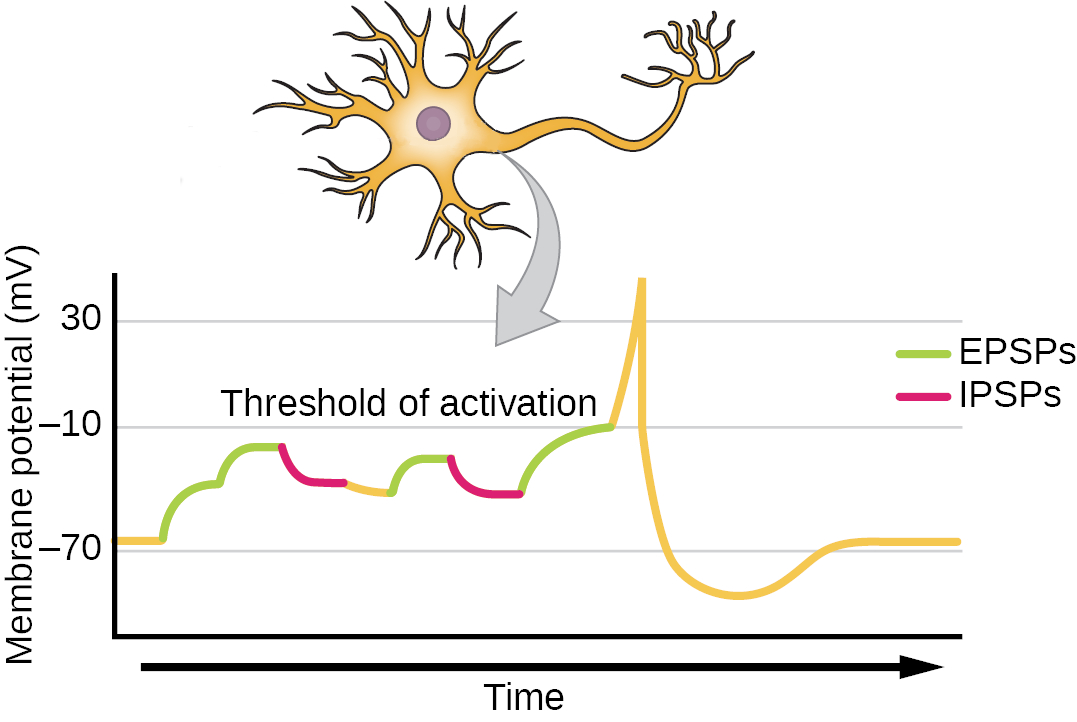
\includegraphics[height=150px]{gfx/Biological_Neuron_edited.jpg}
		\caption{Representation of a biological Neuron\\
			\cite{biology} edited}
		\label{fig:neuron1}
	\end{minipage}\hfill
	\begin{minipage}{0.45\textwidth}
		\centering
		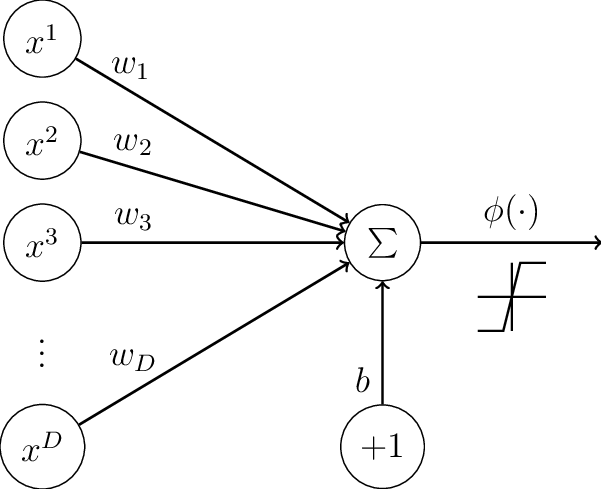
\includegraphics[height=150px]{gfx/Abstract_Neuron.png}
		\caption{Abstraction of a Neuron\\
			\cite{abstract_neuron}}
		\label{fig:neuron2}
	\end{minipage}
\end{figure}

\subsection{Layers}
An individual neuron is too simple to model any complex relations between inputs and outputs. However, certain aggregations of neurons possess the ability to universally approximate functions between input and output.\cite{Approximator}\\
At the core of of conventional neural networks is the idea to collect the signal, many different neurons produce for a given input and reuse them as new features for another round
of neurons. Such a collection is called a \textbf{layer}, and especially a \textbf{hidden layer} if it is neither the input representation nor last in a given network.
A layer is defined by the structure of connections it prescribes. The layers used in this thesis consist of:

\begin{itemize}
	\item \textbf{Input}\\
	The numeric representation of data points can be thought of as outputs of an input-layer. In
	applications, this layer primarily describes assumptions on the shape of the data points. \\
	\item \textbf{Fully-Connected | Dense}\\
	In a fully connected layer, each neuron receives all features of the input, which renders it the most general layer.  In theory, it can learn to effectively drop any number of connections, thus reducing to any kind of the subsequent layers, but establishing such behavior through training might be unfeasible. Besides, it would produce enormous computational overhead. The need for more specialized layers motivated this way, is confirmed by their success throughout various fields.
	Additionally and analogous to the naming of the matrices which implement the computation of neural networks, a fully-connected layer is also called dense.\\
	The sole parameter of a dense layer is the number of neurons it contains. Nonetheless, the parameters of the neurons are still necessary during implementation.\\
	\item \textbf{Convolution}\\
	Inspired by the convolution kernels used in image processing, a convolutional layer combines features of a relatively small neighborhood into a single output.\footnote{In practice, many convolutional layers employ multiple kernels at the same time, meaning that one neighborhood produces numerous outputs. This procedure extends the dimension of the processed data by an additional axis, often called \textbf{channels}. These channels receive special treatment quite often.} This process needs a specification of the data's dimensionality and places an implicit bias on local features. \\
	Convolutions primarily differ in the neighborhood size they define and through the fashion in which they handle missing values at the edges of their data. For example, points beyond the edge of an image could either be defined to be black, white, or even equal to the mean or median of the available part of the convolution. Additionally, contemporary networks utilize \textbf{striding}, where the neighborhods of some features are skipped.\\
	\item \textbf{Pooling}\\
	A pooling layer contains no trainable weights and functions more like a data-processing-step between other layers than anything else. It operates much like a convolutional layer with fixed weights and striding,  replacing a whole neighborhood by a single output, thus reducing the size of the data.\\
	\item \textbf{Flatten}\\  
	Similar to the pooling, a flatten layer specifies a data-processing-step inside a network. It collapses all values of a data point into a single dimension and is the canonical method to prepare multidimensional data for a dense layer. Usually, no parameters are necessary to define a flatten layer.\\
\end{itemize}

\subsection{Architectures}
The collection of layers, and the parameters that define them, is called \textbf{architecture}. In contrast to the term network, an architecture does generally not include the specific trainable weights. However, weights having values close to zero can change the effective shape of an architecture.
As this work aims to enable the reproduction of its results and discusses multiple architectures, a transparent system to note them precisely is fundamental. The architecture description we deploy first declares all default assumptions on its layers. Afterward, a list of layers follows defining the type of said layers, their remaining parameters, and especially the dimensionality of their outputs. Additionally and in the interest of compatibility, the notation remains close to the functional Keras-API utilized throughout the associated source code.\\
The following two examples illustrate the notation:

\subsection*{1}
\begin{figure}[h]
	\centering
	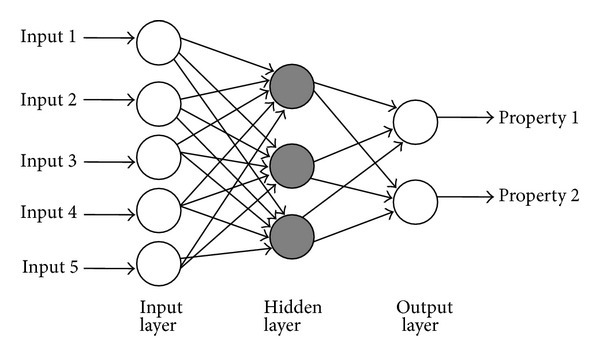
\includegraphics[height=200px]{gfx/Dense_FFNetwork.jpg}
	\caption{Architecture of a small fully-connected network\\
		\cite{dense_network}}
	\label{fig:FFNetwork}
\end{figure}
\begin{tabularx}{\textwidth}[!h]{X X X}
	\multicolumn{3}{c}{\textbf{Simple-FCN | \ref{fig:FFNetwork}}}\\
	\\
	\hline
	\endhead
	\textbf{Defaults} & Dense: activation & rectified linear unit\\
	\hline
	\textbf{Input} & output dimension & 5\\
	[8pt]
	\textbf{Dense} & output dimension & 3\\
	[8pt]
	\textbf{Dense} & output dimension & 2\\
	& activation & softmax\\
	\hline
\end{tabularx}

\newpage

\subsection*{2}

\begin{figure}[h]
	\centering
	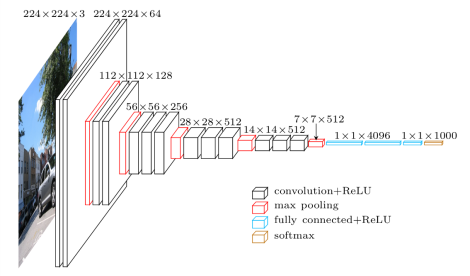
\includegraphics[height=200px]{gfx/vgg16.png}
	\caption{Macroarchitecture of VGG16\\
		\cite{VGG16}}
	\label{fig:VGG16}
\end{figure}
\begin{tabularx}{\textwidth}{X X X}
	\multicolumn{3}{c}{\textbf{VGG-16 | \ref{fig:VGG16}}}\\
	\\
	\hline
	\endhead
	\textbf{Defaults} & Convolution: kernel size & [3,3]\\
	& Convolution: stride & [1,1]\\
	& Convolution: padding & same dimension\\
	& & zero padding\\
	& Convolution: activation & rectified linear unit\\
	& Dense: activation & rectified linear unit\\
	& Softmax: kernel size & [2,2]\\
	& Softmax: stride & [1,1]\\
	\hline
	\textbf{Input} & output dimension & [224,224|3]\\
	[8pt]
	2x \textbf{Convolution} & output dimension & [224,224|64]\\
	[8pt]
	\textbf{Max-Pooling} & output dimension & [112,112|64]\\
	[8pt]
	2x \textbf{Max-Pooling} & output dimension & [112,112|128]\\
	[8pt]
	\textbf{Max-Pooling} & output dimension & [56,56|128]\\
	[8pt]
	3x \textbf{Convolution} & output dimension & [56,56|256]\\
	[8pt]
	\textbf{Max-Pooling} & output dimension & [28,28|256]\\
	[8pt]
	3x \textbf{Convolution} & output dimension & [28,28|512]\\
	[8pt]
	\textbf{Max-Pooling} & output dimension & [14,14|512]\\
	[8pt]
	3x \textbf{Convolution} & output dimension & [14,14|512]\\
	[8pt]
	\textbf{Max-Pooling} & output dimension & [7,7|512]\\
	[8pt]
	\textbf{Flatten} & output dimension & 25.088\\
	[8pt]
	\textbf{Dense} & output dimension & 4096\\
	[8pt]
	\textbf{Dense} & output dimension & 4096\\
	[8pt]
	\textbf{Dense} & output dimension & 1000\\
	& activation & softmax\\
	\hline
\end{tabularx}


\section{Pruning}
As the computational power of modern devices increases ever larger architectures become possible. While this allows for more precise models on any given data it is important to recall that pure representation is not the ultimate goal of most applications.\\
All tasks discussed in this work can be categorized as \textbf{supervised learning}, meaning they provide a collection of labelled data points and demand an extrapolation of the implicit labelling process, also called \textbf{generalization}.
It is a well known phenomenon in the field of supervised learning\footnote{called \textbf{overfitting}} that generalization suffers from over-adaptation to the given data, which tends to happen more easily in bigger architectures. On the other hand, massive parametrization does not only enable us to approximate the labeling process more precisely but also to find such an approximation feasibly.\cite{Overparametrization}\\
\textbf{Pruning} describes the removal of parts from a trained model, which are estimated to be superfluous after learning. Many researchers have developed pruning methods that achieve a significant reduction in network size with little impact on its performance. Chapter \ref{ch:relatedwork} presents a few such techniques.

\section{Non-Numerical Data}
While many phenomena under research, such as digital images or sound recordings, are inherently well representable in numeric terms, others, such as words or sentences in natural language, are not. Before a network can process such data points, they have to be encoded
Generally, there are two ways to do so:
\begin{itemize}
	\item \textbf{One-Hot-Encoding :}\\
	A one-hot-encoding contains a feature for each possible data point. The value in the corresponding dimension is non-zero if, and only if, the feature fully represents the data.
	If, for example, a vocabulary of size $n$ is given its $m$-th word can be described as a vector with $n$ entries where only the $m$-th entry is non-zero.\\
	\item \textbf{Embedding :}\\
	
	Inspired by the way humans can describe various through the use of numerical values in relatively few feature-dimensions, embeddings assign each data point a numerical vector in a space with arbitrary features. If its dimension is significantly lower than the size of the dataset, the embedding describes the data much more efficiently. However, there is no inherent guarantee that this representation retains the information present; In contrast to the one-hot-encoding, which at least remains humanly legible, implying the presence of said information. To avoid its loss, researchers have applied different restrictions to the way data points are distributed in this arbitrary space.
	In contemporary work about natural language processing, embeddings, where a neural network learned the distribution of words in such a space, have become a useful tool for preprocessing. \cite{Word2Vec}
\end{itemize} 

\section{Preprocessing for Natural Language Processing}
In addition the previously mentioned treatment for any dataset there are additional preprocessing steps when handling text-inputs in \textbf{natural language}\footnote{The term natural language describes language written, spoken and otherwise used by humans in contrast to precisely defined languages used for communication between computation devices.}. The most important ones are \textbf{tokenization}, the separation of a text into words and/or sentences, and \textbf{stopword removal}, the removal of little to no syntactic or semantic importance.\\
As the former is almost always necessary to even quantify the numeric representation of the datapoints most frameworks provide datasets already preprocessed in such a manner.\\
The later is a canonical inclusion into any natural-language-processing data-flow but also is generally not preemptively applied to dataset.